\documentclass[a4paper,12pt]{report}
\usepackage[utf8]{inputenc}
\usepackage{graphicx} % Para incluir imágenes
\usepackage{tocloft} % Para personalizar índices
\usepackage{hyperref} % Para enlaces
\usepackage{titlesec} % Para personalizar títulos
\usepackage[backend=biber,style=ieee]{biblatex} % Bibliografía con biblatex
\usepackage{subcaption} % Para el collage de imagenes

\usepackage{indentfirst} % Para la sangria

\usepackage{ragged2e}

\usepackage{amsmath} % Pack Nomenclatura Matemática
\usepackage{amsmath, amssymb}
\usepackage{bm}


% INDICE ------------------------------------------------------

% Cambiar título del índice
\renewcommand{\contentsname}{Índice General}

% Personalizar el formato de capítulos en el índice
\renewcommand{\cftchapleader}{\cftdotfill{\cftdotsep}} % Puntos entre títulos y números
\renewcommand{\cftchapdotsep}{1.5} % Ajusta la separación entre puntos

% CAPITULOS ---------------------------------------------------

% Redefinir el formato del capítulo y eliminar el espacio superior
\titleformat{\chapter}[block]
    {\normalfont\LARGE\bfseries\centering} % Estilo: tamaño grande, negrita, centrado
    {} % Sin prefijo como "Chapter"
    {0pt} % Sin espacio entre el prefijo y el título
    {\LARGE} % Estilo del título del capítulo
\titlespacing*{\chapter}{0pt}{-50pt}{20pt} % Ajustar espaciado: elimina espacio superior

% BIBLIOGRAFÍA -----------------------------------------------------

% Carga el archivo .bib
\addbibresource{bibliografia.bib} % Archivo con las referencias

% SANGRÍA -----------------------------------------------------
\setlength{\parindent}{15pt} % Añade la sagría como tal
\setlength{\parskip}{10pt} % Añade espacio entre párrafos
% -------------------------------------------------------------
\begin{document}
\justifying
% Portada
\begin{titlepage}
    \thispagestyle{empty} % Sin numeración ni encabezado
    \begin{center}
    \centering
    \vspace*{-3cm} % Espaciado superior
    \includegraphics[width=1\textwidth]{images/logo-uax.png} % Logo opcional
    \vspace{1cm}

    {\large \textbf{UNIVERSIDAD ALFONSO X EL SABIO}} \\[0.5cm] % Título principal
    {\large \textbf{FACULTAD BUSINESS AND TECH}} \\[1cm] % Título principal

    {\LARGE \textbf{
    Estudio de los fenotipos \\[0.3cm]
    conductuales, la persistencia y la\\[0.3cm]
    cooperación en redes a través de\\[0.3cm]
    teoría de juegos
    }} \\[1.3cm]

    {\large \textbf{Miguel González González}} \\[3 cm]

    {\Large \textbf{TRABAJO DE FIN DE GRADO}} \\[0.5cm]
    {\Large \textbf{GRADO EN INGENIERÍA MATEMÁTICA}}
    

    \vfill % Para alinear el texto al final de la página
    \textbf{Villanueva de la Cañada, 2025} \\

    \vspace*{1cm}
    \end{center}
\end{titlepage}
\newpage

\begin{titlepage}
    \thispagestyle{empty}
    \begin{center}
        \vspace*{-2.5cm}
        \includegraphics[width=0.18\textwidth]{images/logo_blanco_y_negro.png}

        \vspace{1cm}
        {\bfseries\Large UNIVERSIDAD ALFONSO X EL SABIO}

        \vspace{1.5cm}
        {\large \textbf{Grado en Ingeniería Matemática}}

        \vspace{2.5cm}
        {\LARGE \textbf{
        Estudio de los fenotipos \\[0.3cm]
        conductuales, la persistencia y la\\[0.3cm]
        cooperación en redes a través de\\[0.3cm]
        teoría de juegos
        }} \\[1.3cm]
    \end{center}    
    \vspace{2.5cm}
    {\large \textbf{ALUMNO:} Miguel González González} \\[0.5cm]
    {\large \textbf{NP:} 138683} \\[0.5cm]
    {\large \textbf{TUTOR DEL TRABAJO:} Hugo Andrea Galindo Beleña} \\[0.5cm]        
    {\large \textbf{FECHA DE PRESENTACIÓN:} Junio de 2025} \\[0.5cm]        
    \textbf{Firma del director:}
    \hfill
    \textbf{Firma del alumno:}
\end{titlepage}


% Índices
\newpage
\tableofcontents % Índice general

\newpage

% ------------------------------------------------------------

% Introducción
\chapter{Introducción}

Los seres humanos, como seres sociales y racionales, se ven involucrados de manera involuntaria en interacciones sociales en las que los implicados actúan de manera estratégica. Del mismo modo, los individuos implicados anticipan las posibles respuestas de los demás actores, buscando el resultado que más les favorece.

Algunas de estas interacciones sociales incluyen dilemas, donde el interés propio y el colectivo se ven enfrentados, conflicto entre la racionalidad individual y colectiva, entre intereses propios a corto plazo e intereses colectivos a largo plazo \cite{dawes1980social,kollock1998social,vanLange2013psychology}. Estos y otros escenarios han sido estudiados en economía, psicología y sociología, utilizando un marco teórico para comprender como los actores acometen cooperación o conflicto.

La Teoría de Juegos tradicional se basa en que los actores son racionales y egoistas en su totalidad, pero sabemos que las personas no siempre son totalmente racionales, es decir, que no siempre se persiguen objetivos meramente egoistas.
Es así como se introduce la nueva Teoría de Juegos conocida como Teoría de Juegos Conductual\cite{camerer2003behavioral,kagel1995handbook},y posteriormente la Evolutiva\cite{sigmund2010calculus,gintis2009game}, que ya no solamente trata a los tomadores de decisiones como racionales egoistas, sino que incorporan factores psicológicos, racionalidad imperfecta, capacidad de aprendizaje y experiencias, además de ser capaces de cooperar cuando la teoría predice lo contrario.

Estos y otros trabajos han respaldado que la racionalidad no es suficiente para predecir el comportamiento humano, ya que la cooperación puede surgir sin necesidad de un plan centralizado. La cooperación también depende de la situacion de los decisores, importando mucho la información de la que disponen, el contexto de las decisiones y las estrategias de cada uno \cite{sigmund2010calculus,gintis2009game,myerson1991game}.

En este contexto, resulta interesante analizar cómo distintas disposiciones estratégicas conviven y evolucionan dentro de una población. En vez de dar por sentado que todos los individuos actuan de manera homogenea, varios estudios han identificado la existencia de fenotipos conductuales consistentes, que guian las decisiones en dilemas sociales \cite{paper_principal}. Añadir tal diversidad estratégica permite una aproximación más realista a los modelos de comportamiento, buscando nuevas formas de entender fenómeos como la aparición espontanea de cooperación o la resistencia al cambio.

\newpage

Este Trabajo de Fin de Grado propone un modelo basado en la teoría de juegos evolutiva, en el que una población de agentes heterogéneos  interactúa de manera local sobre una retícula periódica. Cada jugador sigue un comportamiento estratégico asociado a su fenotipo, además de un nivel de persistencia que condiciona su capacidad de adaptación. A través de simulaciones, se estudia cómo el contexto loca y global,y los parámetros que regulan el cambio influyen en la dinámica colectiva del sistema.

El objetivo principal es qué configuraciones favorecen a la cooperación sostenida en el tiempo, variando las distribuciones de los fentoipos, identificar qué fenotipos tienden a prevalecer bajo distintas condiciones y analizar que tan estable es el sistema ante perturbaciones. Este trabajo no solamente trata de replicar el comportamiento observado de manera empírica, sino también trata de ofrecer un marco flexible para comprender mejor la complejidad ligada a los procesos de decisión social.

% ------------------------------------------------------------
% Revisión de la literatura
\chapter{Revisión de la literatura}

Dentro del campo de la Teoría de Juegos, hay muchos estudios que hablan sobre las decisiones irracionales que toman ciertos individuos en situaciones estratégicas colectivas, incluso cuando la respuesta óptima para el individuo era clara. Esto se debe a que no todos los seres humanos somos racionales y egoístas en su totalidad, y dependemos de otros factores como la moralidad, la confianza o el conocimiento para tomar decisiones \cite{dawes1980social}. Hay veces que estas malas decisiones se deben a un nivel cognitivo bajo, pero en otras ocasiones, se trata de un dilema mayor o dilema social, en el cual las decisiones contraponen el bien individual y el colectivo \cite{kollock1998social}.

Los dilemas sociales han sido estudiados en muchos contextos diferentes y con muchas variantes, para poder entender qué factores influyen en las negociaciones y en qué circunstancias se da la cooperación. La cooperación no depende solamente de la racionalidad, hay muchas otras variables que complican el estudio de la posible cooperación entre dos individuos, como por ejemplo: reciprocidad, equidad, contexto, obligaciones morales, conocimientos, razonamientos estratégicos, experiencias pasadas, entre muchas otras \cite{sigmund2010calculus,camerer2003behavioral,kagel1995handbook,gintis2009game}.

El punto es, que hay individuos que aún dándoles razones suficientes para no cooperar, cooperan contra sus propios beneficios. Pareciera que el hecho de cooperar o no en estos dilemas sociales fuera más allá de todas las variables previamente mencionadas, como si fuera algo intrínseco de cada individuo.

Existe un estudio que avala este punto de vista, dando la conclusión de la existencia de cuatro fenotipos conductuales en los juegos diádicos como el del dilema del prisionero \cite{paper_principal}. Estos cuatro fenotipos fueron definidos de la siguiente manera:

\begin{itemize}
\item \textbf{Envidioso:} Quiere obtener mejor resultado que su oponente, sin importar si ello implica una menor ganancia total.
\item \textbf{Optimista:} Pretende buscar el mejor resultado mutuo posible, incluso si esto perjudica a su ganancia individual.
\item \textbf{Pesimista:} Evita el peor resultado, eligiendo siempre lo más seguro y suponiendo el peor escenario como el más probable.
\item \textbf{Confiado:} Siempre busca la cooperación y espera lo mismo de su oponente.
\end{itemize}

También existe un quinto fenotipo, conocido como indefinido, que representa a aquellos individuos cuyo comportamiento no sigue a una estrategia clara o coherente. Este tipo de jugador actúa de forma aleatoria, lo que introduce un elemento de incertidumbre en las dinámicas del juego. Aunque minoritario, su presencia puede alterar la evolución del sistema y a su vez la dinámica de cooperación que debería seguir \cite{paper_principal}.

Este artículo nos puede llevar a la conclusión de que, en escenarios estratégicos con dilemas sociales, se puede predecir el comportamiento humano. La identificación de fenotipos estratégicos recurrentes sugiere que es posible anticipar, al menos de manera parcial, las decisiones de los individuos en contextos de interacción estratégica. Esto abre la puerta a modelos conductuales más ajustados a la realidad, que incorporan la diversidad de perfiles y la influencia del entorno.

Existe otro estudio que habla de la persistencia de las estrategias que siguen los individuos en entornos locales frente a globales, donde los actores adaptan su nivel de persistencia comparando la situación local frente a la global \cite{liming2022adaptative}. Los individuos mantendrán o cambiarán su estrategia en función de si su rendimiento local es mejor que el rendimiento medio global.

Esta práctica lleva a mejorar los niveles de persistencia entre los cooperadores promoviendo la cooperación en juegos evolutivos, cosa que de no ser por estas comparativas de entornos sería complicado de mantener porque los agentes egoístas tienen más incentivos para actuar de una manera oportunista. En ausencia de este tipo de análisis comparativo, la sostenibilidad de la cooperación sería mucho más difícil de alcanzar, dado que los agentes con estrategias egoístas suelen presentar mayores incentivos inmediatos para adoptar comportamientos oportunistas.

Hay veces, que en estos juegos diádicos la cooperación no es la mejor estrategia, y en otras situaciones como en las sociedades humanas, la cooperación y coordinación entre los actores promueven el surgimiento y mantenimiento de las sociedades, poniendo como ejemplo a Japón. Existen conceptos que fomentan estas prácticas, como la de la "reciprocidad institucionalizada" que implica incorporar la estrategia recíproca como institución formal para facilitar la cooperación y reducir la probabilidad de comportamientos oportunistas \cite{Ozono2016Reciprocity}.

Como sociedad, es importante colaborar y cooperar para promover y mantener la comunidad, pero dentro de las comunidades existe más de un tipo de fenotipo, no solamente los colaboradores y los oportunistas, siendo un dilema la siguiente cuestión: ¿Hasta que punto afecta que una comunidad sea más o menos colaborativa? ¿Se desarrollará de una mejor forma una comunidad con una mayoría de un fenotipo mejor que otra? ¿Qué tipos de fenotipos son capaces de convivir mejor dentro de una comunidad y cuáles en cambio provocarán que su entoro tenga un peor rendimiento? 

% ------------------------------------------------------------
% Formulación matemática / Modelo
\chapter{Formulación matemática}

Para el modelo matemático, vamos a simular una población a través de una combinación entre el método de Monte Carlo y una retícula periódica.
La Simulación de Monte Carlo es una técnica matemática que usa números aleatorios y probabilidad para entender el impacto del riesgo de un modelo en la realidad.
En este caso, el modelo será una población dividida en vecindarios o vecinos los cuales solo interactuarán entre ellos, mezclando fenotipos en unos vecindarios y dejando vecindarios de otros fenotipos de mayoritariamente.
Las interacciones se basan en juegos de la Teoría de Juegos estáticos con pesos aleatorios.
Con este modelo trataremos de entender cómo las perturbaciones aleatorias se propagan al resto del modelo.

\section{Marco del Modelo Matemático}

Consideramos una población de individuos dispuestos sobre una retícula de tamaño \( L \times L\), con condiciones de periodicidad en los bordes. Cada nodo representa un único jugador que interactua solamente con sus vecinos adyacentes.
A cada jugador \( i \) se le asigna una estrategia fenotípica o fenotipo estratégico la cual puede evolucionar durante la simulación. Los fenotipos que existen en la simulación son:

\[
\Psi = \{ \text{Envidioso (E)}, \text{Optimista (O)}, \text{Pesimista (P)}, \text{Altruista (A)}, \text{Aleatorio (R)} \}
\]

Cada interacción entre individuos se modela como un juego \( 2 \times 2 \), con la siguiente matriz de pagos:

\[
\begin{array}{c|cc}
  & C & D \\
\hline
C & 1 & S \\
D & T & 0 \\
\end{array}
\quad \text{donde } 0 \leq T \leq 2, \quad -1 \leq S \leq 1
\]

Los jugadores eligen entre cooperar (C) o traicionar (D), siguiendo una de las siguientes reglas fenotípicas:

\newpage


\begin{figure}[h!]
    \centering
    \includegraphics[width=1\textwidth]{images/fenotipos_modelo_teorico.png}
    \label{fig:fenotipos-modelo}
    \caption{Modelo teórico de los fenotipos}
\end{figure}

Cada jugador adopta una estrategia en función del contexto del juego en el que se encuentra. Denotamos por \( s \in  S \)  al estado del juego o situación estratégica percibida por el jugador, la cual incluye la información relevante para su toma de decisiones. En nuestro caso, este estado está determinado por los valores de los parámetros de la matriz de pagos: la tentación \( T \), el castigo \( 0 \), la recompensa mutua \( 1 \), y el valor de \( S \), que representa la ganancia al cooperar frente a un oponente traidor. Así, cada fenotipo puede ser descrito como una función de decisión
\[
\psi : S \rightarrow \{C, D\}
\]
donde \( \psi(s) \) devuelve la estrategia elegida (cooperar \( C \) o traicionar \( D \)) según el tipo de jugador y el estado \( s \) percibido.


\begin{itemize}
  \item \textbf{Envidioso (E):} Coopera solo si recibe un pago mayor que el del oponente:
  \[
  E(s) =
  \begin{cases}
    C & \text{si } S > T \\
    D & \text{si } S \leq T
  \end{cases}
  \]

  \item \textbf{Optimista (O):} Busca maximizar su beneficio:
  \[
  O(s) =
  \begin{cases}
    C & \text{si } T < 1 \\
    D & \text{si } T > 1
  \end{cases}
  \]

  \item \textbf{Pesimista (P):} Minimiza el riesgo, esperando el peor escenario:
  \[
  P(s) =
  \begin{cases}
    C & \text{si } S > 0 \\
    D & \text{si } S \leq 0
  \end{cases}
  \]

  \item \textbf{Altruista (A):} Coopera incondicionalmente:
  \[
  A(s) = C
  \]

  \item \textbf{Aleatorio (R):} Coopera o traiciona con igual probabilidad:
  \[
  R(s) =
  \begin{cases}
    C & \text{con probabilidad } \frac{1}{2} \\
    D & \text{con probabilidad } \frac{1}{2}
  \end{cases}
  \]
\end{itemize}
\justifying
A cada fenotipo \( \psi_i \in \Psi \) se le asocia una regla de comportamiento \( \mathcal{R}_{\psi^\alpha} \), que determina la probabilidad estratégica o la elección estratégica del jugador en función del contexto del juego y del entorno.

Podemos representar la probabilidad de cooperación de un jugador con fenotipo \( \psi^\alpha \) en el tiempo \( t \) como:

\[
P_i(t) = \mathbb{P}(s_i(t) = C \mid \psi_i = \psi^\alpha, \mathcal{G}_i(t))
\]

donde \( \mathcal{G}_i(t) \) representa el estado del juego percibido por el jugador \( i \).

Al inicio del modelo, cada jugador es asignado a un fenotipo de acuerdo a una distribución de probabilidad con:

\[
\mathbb{P}(\psi_i = \psi^\alpha) = \pi_\alpha, \quad \sum_{\alpha=1}^{M} \pi_\alpha = 1
\]

Las probabilidades de cada fenotipo vienen determinadas por "Humans display a reduced set of consistent behavioral phenotypes in dyadic games "\cite{paper_principal}. Estas probabilidades son:

\begin{center}
\small
\begin{tabular}{l}
\textbf{Envidioso}: 30\% \\
\textbf{Pesimista}: 21\% \\
\textbf{Optimista}: 20\% \\
\textbf{Confiado}: 17\% \\
\textbf{Indefinido}: 12\% \\
\end{tabular}
\end{center}

Cada jugador posee un nivel de persistencia el cual puede variar con el tiempo \(t\), denotado por \( \tau_i(t) \in [\tau_D, \tau_U] \). Además se introduce un contador \( \theta_i \), que registra cuántos pasos lleva el jugador manteniendo su estrategia actual.

Definimos el entorno local del jugador \( i \) como una función \( \phi_i(t) \) que depende de los fenotipos de sus vecinos:

\[
\phi_i(t) = \frac{1}{k_i} \sum_{j \in \mathcal{N}_i} f(s_j(t))
\]

donde \( \mathcal{N}_i \) es el conjunto de vecinos inmediatos de \( i \), \( k_i = |\mathcal{N}_i| \), y \( f(\cdot) \) es una función que mapea el fenotipo a una medida cuantificable de cooperación.

Asimismo, se define el entorno global \( \phi(t) \) como:

\[
\phi(t) = \frac{1}{N} \sum_{j=1}^{N} f(s_j(t))
\]

Cada jugador compara su entorno local con el global. Si \( \phi_i(t) > \phi(t) \), se considera que se encuentra en un entorno favorable y tenderá a aumentar su nivel de persistencia. De lo contrario, lo disminuirá. Esta dinámica se implementa mediante una función tipo Fermi:

\[
P_{\text{incremento}} = \frac{1}{1 + \exp\left( -\frac{ \phi_i(t) - \phi(t) }{K_1} \right)}
\]

donde \( K_1 \) es un parámetro de ruido que controla la sensibilidad a las diferencias de entorno.

Para modelar estos cambios de forma gradual, se introduce el parámetro \( \Delta\tau > 0 \), que controla el incremento o decremento del nivel de persistencia. Así, si el entorno es favorable ,es decir, el jugador decide aumentar su persistencia, el valor se actualiza como:

\[
\tau_i(t+1) = \min(\tau_i(t) + \Delta\tau, \tau_U)
\]

Y si el entorno es desfavorable, la actualización es:

\[
\tau_i(t+1) = \max(\tau_i(t) - \Delta\tau, \tau_D)
\]

Este mecanismo permite que los jugadores ajusten de forma progresiva su resistencia al cambio de estrategia, dependiendo de la calidad relativa de su entorno local.

Los jugadores solo consideran cambiar su estrategia cuando su temporizador alcanza su nivel de persistencia actual: \( \theta_i \geq \tau_i(t) \). En ese momento, el jugador \( i \) selecciona un vecino \( j \) al azar y considera adoptar su fenotipo con una probabilidad dada por:

\[
W_{s_i \leftarrow s_j}(t) = \frac{1}{1 + \exp\left( -\frac{ \pi_j(t) - \pi_i(t) }{K_2} \right)}
\]

donde \( \pi_i(t) \) y \( \pi_j(t) \) son los pagos acumulados de \( i \) y \( j \), respectivamente, calculados a partir de sus interacciones con sus vecinos, y \( K_2 \) es otro parámetro de ruido.

Una vez imitada la estrategia, el temporizador del jugador se reinicia: \( \theta_i = 0 \). Este mecanismo representa que el individuo ha adoptado un nuevo fenotipo y, por tanto, necesita un nuevo periodo de observación antes de poder plantearse otro cambio. En caso de que no imite al vecino seleccionado, su temporizador aumenta en una unidad, acumulando pasos hasta alcanzar nuevamente su nivel de persistencia \( \tau_i \). Esta dinámica garantiza que los jugadores no cambien de estrategia de manera impulsiva, introduciendo una memoria temporal que modula la frecuencia de los cambios.


% Resultados y discusión
\chapter{Resultados y discusión}

Basandonos en el modelo matemático propuesto en el apartado anterior, crearmos un programa que sigue la simulación de Monte Carlo como es propuesta en el marco teórico \cite{TFG_SimulacionAgentesFenotipos}.
Una vez probado el modelo lo utilizamos para hacer diversas simulaciones, alterando los parámetros y observando qué patrones o ciclos encontramos dados unos parámetros concretos.
Tratamos de entender el funcionamiento de los fenotipos en diferentes entornos, ya sean vecindarios predeterminados como distribuciones o parámetros de ruido varios.
Salvo en simulaciones concretas, la distribución de la retícula será aleatoria, es decir, que las reticulas distribuirán siguiendo las probabilidades establecidas las posiciones de los fenotipos de manera aleatoria. Esto es importante ya que independientemente de que una simulación con ciertos valores para los diferentes parámetros nos de un resultado similar puede suceder que tengamos una distribución que favorezca la progresión de algún fenotipo que no debería progresar.

\vspace{1.5em}
\noindent\textbf{Probabilidades basadas en el marco teórico}
\vspace{0.5em}


Las primeras simulaciones se diseñaron para reproducir el contexto empírico descrito en el artículo “Humans display a reduced set of consistent behavioral phenotypes in dyadic games” \cite{paper_principal}, el cual identifica una distribución específica de fenotipos conductuales en experimentos con humanos. En este caso, se utilizó dicha distribución como configuración inicial en la retícula, combinada con parámetros de sensibilidad \( K_1 = 0.1 \) y \( K_2 = 0.1 \), que regulan respectivamente la adaptación del nivel de persistencia y la probabilidad de imitación entre jugadores.

% Collage de simulación
%TOP
\begin{figure}[h]
    \centering
    \begin{minipage}{0.49\textwidth}
    \centering
    \includegraphics[width=1\textwidth]{images/prob_normal/SIM1/fenotipos_evolucion.png}
    \label{fig:fenotipos-sim1}
    \end{minipage}
    \hfill
    \begin{minipage}{0.49\textwidth}
    \centering
    \includegraphics[width=1\textwidth]{images/prob_normal/SIM1/cooperacion_global.png}
    \label{fig:cooperacion-sim1}
    \end{minipage}
    \caption{Simulación 1}
\end{figure}

Observamos en la imagen de la evolución de la proporcion de fenotipos, que a lo largo de 50 iteraciones la proporción de los fenotipos experimenta cambios notables. Aunque algunos fenotipos como el optimista y el envidioso presentan una dinámica más activa, el fenotipo aleatorio tiende a reducirse progresivamente, lo cual es coherente con su falta de consistencia estratégica frente a los otros perfiles. En paralelo, la cooperación global presenta un comportamiento oscilante con una ligera tendencia descendente en la fase intermedia, lo que indica que la retícula no alcanza un estado estable de cooperación alta.

%UNDER
\begin{figure}[h]
    \centering
    \begin{subfigure}[t]{0.49\textwidth}
        \centering
        \includegraphics[width=1\textwidth]{images/prob_normal/SIM2/fenotipos_evolucion.png}
        \label{fig:enter-label}
    \end{subfigure}
    \hfill
    \begin{subfigure}[t]{0.49\textwidth}
        \centering
        \includegraphics[width=1\textwidth]{images/prob_normal/SIM2/cooperacion_global.png}
        \label{fig:enter-label}
    \end{subfigure}
    \caption{Simulación 2}
\end{figure}

Con el objetivo de analizar con mayor profundidad la influencia de los parámetros de sensibilidad, se realizaron simulaciones adicionales modificando \( K_1 \) y \( K_2 \) de forma independiente. En primer lugar, se exploraron distintos valores de \( K_1 \), el cual determina qué tan sensible es un jugador al comparar su entorno local con el entorno global. Este parámetro regula la probabilidad de que aumente o disminuya su nivel de persistencia. A menor valor de \( K_1 \), la función tipo Fermi que rige el ajuste de \( \tau \) se vuelve más abrupta, lo que conlleva decisiones más reactivas ante diferencias sutiles. A mayor \( K_1 \), el cambio de persistencia es más gradual, favoreciendo la estabilidad.

\newpage

\subsection*{Simlaciones variando el parámetro \( K_1 \)}

Para las simulaciones del parámetro \( K_1 \), los valores de el parámetro \( K_2 \) serán siempre 0.1 durante este apartado.

\vspace{1.5em}
\noindent\textbf{Parámetro \( K_1\) con valor 0.01}
\vspace{0.5em}

Para explorar el efecto de una alta sensibilidad de los jugadores ante diferencias entre su entorno local y global, se realizaron simulaciones fijando el parámetro \( K_1 \) en un valor bajo: 0.01. Este valor acentúa la pendiente de la función tipo Fermi que regula el ajuste del nivel de persistencia (\( \tau \)), lo que significa que incluso pequeñas diferencias percibidas entre el vecindario y el sistema general provocan cambios abruptos en el comportamiento de los jugadores.


\begin{figure}[h!]
    \centering
    \begin{minipage}{0.49\textwidth}
    \centering
    \includegraphics[width=1\textwidth]{images/K1/001/fenotipos_evolucion.png}
    \label{fig:enter-label}
    \end{minipage}
    \hfill
    \begin{minipage}{0.49\textwidth}
    \centering
    \includegraphics[width=1\textwidth]{images/K1/001/cooperacion_global.png}
    \label{fig:enter-label}
    \end{minipage}
    \caption{Cooperación global con fenotipos equidistribuidos}
\end{figure}

Como se observa en las gráficas, la dinámica del sistema resulta altamente inestable, especialmente a partir de la iteración 120. La cooperación global presenta grandes oscilaciones, y los fenotipos predominantes cambian con frecuencia. Esta falta de estabilidad puede atribuirse a la excesiva reactividad de los jugadores, que ajustan su persistencia de forma continua, impidiendo que se consoliden patrones cooperativos duraderos.

Para evaluar el impacto de la distribución inicial de fenotipos sobre la evolución de la cooperación, se realizaron simulaciones adicionales manteniendo \( K_1 = 0.01 \) pero modificando las proporciones de cada tipo de jugador en la retícula. Se compararon dos escenarios opuestos: uno con mayoría de fenotipos no cooperadores (envidiosos y pesimistas), y otro con mayoría de fenotipos cooperadores (optimistas y altruistas).

%TOP
\begin{figure}[h]
    \centering
    \begin{minipage}{0.49\textwidth}
    \centering
    \includegraphics[width=1\textwidth]{images/K1/001/EP/fenotipos_evolucion.png}
    \label{fig:enter-label}
    \end{minipage}
    \hfill
    \begin{minipage}{0.49\textwidth}
    \centering
    \includegraphics[width=1\textwidth]{images/K1/001/EP/cooperacion_global.png}
    \label{fig:enter-label}
    \end{minipage}
    \caption{Mayoría de Envidiosos y Pesimistas}
\end{figure}

\newpage

En el primer caso, se observa una caída progresiva de la cooperación global, alcanzando niveles mínimos al final de la simulación. Esto se debe a que los fenotipos dominantes no promueven la cooperación, y el entorno volátil impide que los cooperadores puedan mantenerse en la población.


%UNDER
\begin{figure}[h]
    \centering
    \begin{subfigure}[t]{0.49\textwidth}
        \centering
        \includegraphics[width=1\textwidth]{images/K1/001/OA/fenotipos_evolucion.png}
        \label{fig:enter-label}
    \end{subfigure}
    \hfill
    \begin{subfigure}[t]{0.49\textwidth}
        \centering
        \includegraphics[width=1\textwidth]{images/K1/001/OA/cooperacion_global.png}
        \label{fig:enter-label}
    \end{subfigure}
    \caption{Mayoría de Optimistas y Altruistas}
\end{figure}

Por el contrario, cuando se favorece inicialmente la aparición de fenotipos cooperadores, el sistema evoluciona hacia una cooperación global casi perfecta. Se observa cómo los fenotipos optimistas y altruistas tienden a dominar la retícula, desplazando a los perfiles oportunistas y aleatorios. La estabilidad lograda en este caso demuestra que, incluso bajo alta sensibilidad (\( K_1 = 0.01 \)), una buena distribución inicial puede favorecer comportamientos cooperativos sostenidos si los perfiles predominantes comparten expectativas de colaboración.


\newpage

\vspace{1.5em}
\noindent\textbf{Parámetro \( K_1 \) con valor 0.3}
\vspace{0.5em}



Se realizaron simulaciones con el parámetro \( K_1 \) configurado en 0.3, lo que implica una sensibilidad moderada de los jugadores al comparar su entorno local con el global. Esta elección permite una transición más progresiva en el ajuste de la persistencia (\( \tau \)), favoreciendo un equilibrio entre estabilidad y capacidad de adaptación.


\begin{figure}[h!]
    \centering
    \begin{minipage}{0.49\textwidth}
    \centering
    \includegraphics[width=1\textwidth]{images/K1/030/fenotipos_evolucion.png}
    \label{fig:enter-label}
    \end{minipage}
    \hfill
    \begin{minipage}{0.49\textwidth}
    \centering
    \includegraphics[width=1\textwidth]{images/K1/030/cooperacion_global.png}
    \label{fig:enter-label}
    \end{minipage}
    \caption{Cooperación global con fenotipos equidistribuidos}
\end{figure}

Como se muestra en las gráficas, cuando se parte de una distribución equitativa (20\% para cada fenotipo), la dinámica evolutiva favorece el ascenso de los perfiles cooperadores. En concreto, los jugadores altruistas (verde) y optimistas (naranja) aumentan su proporción significativamente a lo largo del tiempo, hasta ocupar la mayoría de la retícula. Como consecuencia, la cooperación global (\( \phi(t) \)) crece de forma progresiva y sostenida, alcanzando valores cercanos a 1.

Este comportamiento indica que, bajo una sensibilidad media, los jugadores son capaces de identificar entornos locales más cooperativos, lo que refuerza su persistencia y favorece la estabilidad del sistema. Además, la baja reactividad evita que los jugadores cambien de fenotipo impulsivamente, lo que permite que las estrategias cooperativas prosperen en el largo plazo.

\newpage

%TOP
\begin{figure}[h]
    \centering
    \begin{minipage}{0.49\textwidth}
    \centering
    \includegraphics[width=1\textwidth]{images/K1/030/EP/fenotipos_evolucion.png}
    \label{fig:enter-label}
    \end{minipage}
    \hfill
    \begin{minipage}{0.49\textwidth}
    \centering
    \includegraphics[width=1\textwidth]{images/K1/030/EP/cooperacion_global.png}
    \label{fig:enter-label}
    \end{minipage}
    \caption{Mayoría de Envidiosos y Pesimistas}
\end{figure}

Por el contrario, en el escenario con mayoría de perfiles no cooperadores, la cooperación global disminuye de forma sostenida, y los fenotipos optimista y altruista desaparecen casi por completo. La retícula se ve dominada por jugadores envidiosos y pesimistas, lo que reduce la probabilidad de establecer vecindarios cooperativos y disminuye la eficacia de los mecanismos de persistencia.


%UNDER
\begin{figure}[h]
    \centering
    \begin{subfigure}[t]{0.49\textwidth}
        \centering
        \includegraphics[width=1\textwidth]{images/K1/030/OA/fenotipos_evolucion.png}
        \label{fig:enter-label}
    \end{subfigure}
    \hfill
    \begin{subfigure}[t]{0.49\textwidth}
        \centering
        \includegraphics[width=1\textwidth]{images/K1/030/OA/cooperacion_global.png}
        \label{fig:enter-label}
    \end{subfigure}
    \caption{Mayoría de Optimistas y Altruistas}
\end{figure}


En el caso de mayoría cooperadora, la cooperación global alcanza rápidamente altos niveles, manteniéndose estable durante toda la simulación. Esto demuestra la eficacia de la configuración cooperativa inicial bajo este valor de sensibilidad, donde las estrategias cooperativas tienen margen para consolidarse gracias a la persistencia y estabilidad local.


\newpage

\vspace{1.5em}
\noindent\textbf{Parámetro \( K_1 \) con valor 0.7}
\vspace{0.5em}

En esta serie de simulaciones se ha establecido el valor del parámetro \( K_1 \) en 0.7, lo que implica que los jugadores presentan una baja sensibilidad a las diferencias entre su entorno local y el entorno global. Esto significa que las variaciones pequeñas en el nivel de cooperación entre vecindarios no son suficientes para provocar un cambio significativo en el nivel de persistencia \( \tau \), resultando en una dinámica más conservadora y estable.

\begin{figure}[h!]
    \centering
    \begin{minipage}{0.49\textwidth}
    \centering
    \includegraphics[width=1\textwidth]{images/K1/070/fenotipos_evolucion.png}
    \label{fig:enter-label}
    \end{minipage}
    \hfill
    \begin{minipage}{0.49\textwidth}
    \centering
    \includegraphics[width=1\textwidth]{images/K1/070/cooperacion_global.png}
    \label{fig:enter-label}
    \end{minipage}
    \caption{Cooperación global con fenotipos equidistribuidos}
\end{figure}

En el caso de una distribución inicial equitativa, como muestran las gráficas, se observa un comportamiento estable durante las primeras fases de la simulación. Aunque algunos fenotipos caen rápidamente —como el pesimista y el aleatorio—, otros como el altruista y el optimista logran aumentar progresivamente su proporción. Como consecuencia, la cooperación global muestra una tendencia ascendente clara, alcanzando valores cercanos a 1 hacia el final del proceso.

Este resultado refleja cómo, bajo baja sensibilidad al entorno, los individuos muestran una alta inercia al cambio, favoreciendo la consolidación de vecindarios cooperativos si estos logran establecerse en etapas tempranas. La cooperación, una vez instaurada, se vuelve robusta frente a pequeñas fluctuaciones.

\newpage

%TOP
\begin{figure}[h]
    \centering
    \begin{minipage}{0.49\textwidth}
    \centering
    \includegraphics[width=1\textwidth]{images/K1/070/EP/fenotipos_evolucion.png}
    \label{fig:enter-label}
    \end{minipage}
    \hfill
    \begin{minipage}{0.49\textwidth}
    \centering
    \includegraphics[width=1\textwidth]{images/K1/070/EP/cooperacion_global.png}
    \label{fig:enter-label}
    \end{minipage}
    \caption{Mayoría de Envidiosos y Pesimistas}
\end{figure}
%UNDER

En el primer escenario, los fenotipos cooperadores comienzan en desventaja. Sin embargo, a diferencia de lo observado en configuraciones con valores más bajos de \( K_1 \), estos fenotipos logran recuperarse y expandirse lentamente conforme avanza la simulación. Este fenómeno se explica por la lentitud en el ajuste de la persistencia, lo que otorga tiempo suficiente para que los cooperadores construyan vecindarios estables incluso desde una posición inicial minoritaria.



\begin{figure}[h]
    \centering
    \begin{subfigure}[t]{0.49\textwidth}
        \centering
        \includegraphics[width=1\textwidth]{images/K1/070/OA/fenotipos_evolucion.png}
        \label{fig:enter-label}
    \end{subfigure}
    \hfill
    \begin{subfigure}[t]{0.49\textwidth}
        \centering
        \includegraphics[width=1\textwidth]{images/K1/070/OA/cooperacion_global.png}
        \label{fig:enter-label}
    \end{subfigure}
    \caption{Mayoría de Optimistas y Altruistas}
\end{figure}

En el segundo caso, los fenotipos cooperadores no solo mantienen su dominio, sino que lo amplían hasta alcanzar una proporción mayoritaria sostenida. La cooperación global sigue una trayectoria ascendente rápida y sostenida, confirmando que bajo condiciones iniciales favorables, una baja sensibilidad al entorno es suficiente para que la cooperación se estabilice y prospere.

\newpage

\vspace{1.5em}
\noindent\textbf{Parámetro \( K_1 \) con valor 1}
\vspace{0.5em}

En esta configuración, se fijó el parámetro \( K_1 \) con un valor de 1.0, lo que implica una sensibilidad muy baja al comparar el entorno local con el global. En este escenario, los jugadores ajustan su nivel de persistencia \( \tau \) de forma muy gradual, de modo que los cambios en la cooperación local deben ser significativos para inducir una modificación en su comportamiento.

\begin{figure}[h!]
    \centering
    \begin{minipage}{0.49\textwidth}
    \centering
    \includegraphics[width=1\textwidth]{images/K1/1/fenotipos_evolucion.png}
    \label{fig:enter-label}
    \end{minipage}
    \hfill
    \begin{minipage}{0.49\textwidth}
    \centering
    \includegraphics[width=1\textwidth]{images/K1/1/cooperacion_global.png}
    \label{fig:enter-label}
    \end{minipage}
    \caption{Cooperación global con fenotipos equidistribuidos}
\end{figure}

Se observa una evolución positiva y sostenida de la cooperación global, que alcanza el valor máximo en torno al paso 200. A lo largo del proceso, los fenotipos cooperadores (optimistas y altruistas) incrementan significativamente su proporción en la retícula. Los fenotipos no cooperadores tienden a desaparecer progresivamente, a excepción de situaciones puntuales de estabilización parcial. La baja sensibilidad favorece este comportamiento, ya que evita reacciones bruscas ante fluctuaciones menores, y permite que las estrategias cooperativas ganen fuerza de forma sostenida.


%TOP
\begin{figure}[h]
    \centering
    \begin{minipage}{0.49\textwidth}
    \centering
    \includegraphics[width=1\textwidth]{images/K1/1/EP/fenotipos_evolucion.png}
    \label{fig:enter-label}
    \end{minipage}
    \hfill
    \begin{minipage}{0.49\textwidth}
    \centering
    \includegraphics[width=1\textwidth]{images/K1/1/EP/cooperacion_global.png}
    \label{fig:enter-label}
    \end{minipage}
    \caption{Mayoría de Envidiosos y Pesimistas}
\end{figure}

También se analizaron escenarios en los que los fenotipos cooperadores comenzaban como minoría, representando un 15\% cada uno (30\% en total). En estos casos, los resultados muestran que, si bien los cooperadores enfrentan inicialmente una mayor dificultad para expandirse, en la mayoría de las simulaciones logran imponerse y dominar la retícula en las últimas fases de la simulación.

%UNDER
\begin{figure}[h]
    \centering
    \begin{subfigure}[t]{0.49\textwidth}
        \centering
        \includegraphics[width=1\textwidth]{images/K1/1/OA/fenotipos_evolucion.png}
        \label{fig:enter-label}
    \end{subfigure}
    \hfill
    \begin{subfigure}[t]{0.49\textwidth}
        \centering
        \includegraphics[width=1\textwidth]{images/K1/1/OA/cooperacion_global.png}
        \label{fig:enter-label}
    \end{subfigure}
    \caption{Mayoría de Optimistas y Altruistas}
\end{figure}

En las simulaciones con una distribución inicial favorable a la cooperación —30\% de optimistas y 30\% de altruistas— el dominio de los fenotipos cooperadores se produce de forma sistemática. La cooperación global alcanza valores cercanos a 1 en fases tempranas, y se mantiene con gran estabilidad.

El entorno inicial favorable, combinado con una baja sensibilidad al entorno, genera condiciones óptimas para el éxito de las estrategias cooperativas. La persistencia elevada evita que los jugadores cambien su fenotipo con facilidad, consolidando de forma temprana un entorno colaborativo.

\newpage

\subsection*{Simlaciones variando el parámetro \( K_2 \)}

Para las simulaciones del parámetro \( K_2 \), los valores de el parámetro \( K_1 \) serán siempre 0.1 durante este apartado.

\vspace{1.5em}
\noindent\textbf{Parámetro \( K_2 \) con valor 0.01}

El parámetro \( K_2 \) regula la probabilidad de imitación del fenotipo de un vecino, en función de la diferencia de pagos acumulados entre jugadores. Un valor bajo como \( K_2 = 0.01 \) representa una alta sensibilidad: pequeñas diferencias en los beneficios obtenidos pueden inducir cambios de fenotipo. Esto genera una dinámica altamente reactiva e inestable.


\begin{figure}[h!]
    \centering
    \begin{minipage}{0.49\textwidth}
    \centering
    \includegraphics[width=1\textwidth]{images/K2/001/fenotipos_evolucion.png}
    \label{fig:enter-label}
    \end{minipage}
    \hfill
    \begin{minipage}{0.49\textwidth}
    \centering
    \includegraphics[width=1\textwidth]{images/K2/001/cooperacion_global.png}
    \label{fig:enter-label}
    \end{minipage}
    \caption{Cooperación global con fenotipos equidistribuidos}
\end{figure}

Como puede observarse en las gráficas, con una distribución equitativa inicial, el sistema no presenta una clara tendencia hacia la cooperación. La cooperación global permanece fluctuante durante toda la simulación, sin alcanzar valores elevados de forma sostenida. Además, los fenotipos indefinidos aumentan su proporción significativamente, lo que sugiere que el sistema está dominado por la aleatoriedad y la falta de consolidación estratégica.

Esto se explica porque la alta sensibilidad produce cambios de fenotipo demasiado frecuentes, impidiendo que los comportamientos cooperativos se afiancen en la retícula. Al ser tan volátiles, incluso los jugadores que cooperan pueden ser reemplazados rápidamente por otros fenotipos menos estables si en un paso concreto su rendimiento es inferior.


%TOP
\begin{figure}[h]
    \centering
    \begin{minipage}{0.49\textwidth}
    \centering
    \includegraphics[width=1\textwidth]{images/K2/001/EP/fenotipos_evolucion.png}
    \label{fig:enter-label}
    \end{minipage}
    \hfill
    \begin{minipage}{0.49\textwidth}
    \centering
    \includegraphics[width=1\textwidth]{images/K2/001/EP/cooperacion_global.png}
    \label{fig:enter-label}
    \end{minipage}
    \caption{Mayoría de Envidiosos y Pesimistas}
\end{figure}

\newpage

En este escenario se parte de una distribución inicial con predominancia de fenotipos no cooperadores (envidiosos y pesimistas). La dinámica del sistema muestra una caída sostenida de la cooperación global y una expansión de estos fenotipos.

Las graficas confirman que la cooperación no se consolida en este entorno. El comportamiento oportunista se impone y los cooperadores (altruistas y optimistas) desaparecen rápidamente. La alta sensibilidad amplifica esta tendencia, ya que los jugadores imitan con facilidad a los fenotipos de mayor beneficio inmediato, lo que perpetúa comportamientos no cooperativos y evita la estabilidad a largo plazo.

%UNDER
\begin{figure}[h]
    \centering
    \begin{subfigure}[t]{0.49\textwidth}
        \centering
        \includegraphics[width=1\textwidth]{images/K2/001/OA/fenotipos_evolucion.png}
        \label{fig:enter-label}
    \end{subfigure}
    \hfill
    \begin{subfigure}[t]{0.49\textwidth}
        \centering
        \includegraphics[width=1\textwidth]{images/K2/001/OA/cooperacion_global.png}
        \label{fig:enter-label}
    \end{subfigure}
    \caption{Mayoría de Optimistas y Altruistas}
\end{figure}

Cuando los fenotipos cooperadores son mayoría desde el inicio, la cooperación logra consolidarse progresivamente, alcanzando niveles cercanos a 1. A pesar de la alta sensibilidad del sistema con \(K_2\) bajo, los cooperadores pueden imponerse si forman vecindarios estables desde las primeras etapas.

\newpage

\vspace{1.5em}
\noindent\textbf{Parámetro \( K_2 \) con valor 0.3}
\vspace{0.5em}

El parámetro \( K_2 \) regula la probabilidad de que un jugador imite el fenotipo de un vecino con mayor beneficio acumulado, y por tanto, su sensibilidad a las diferencias de rendimiento. Un valor intermedio como \( K_2 = 0.3 \) implica que los jugadores no reaccionan impulsivamente a pequeñas diferencias, pero sí son capaces de adaptarse ante rendimientos claramente superiores. Este equilibrio resulta clave para fomentar la estabilidad estratégica sin frenar por completo la evolución de los fenotipos.

\begin{figure}[h!]
    \centering
    \begin{minipage}{0.49\textwidth}
    \centering
    \includegraphics[width=1\textwidth]{images/K2/030/fenotipos_evolucion.png}
    \label{fig:enter-label}
    \end{minipage}
    \hfill
    \begin{minipage}{0.49\textwidth}
    \centering
    \includegraphics[width=1\textwidth]{images/K2/030/cooperacion_global.png}
    \label{fig:enter-label}
    \end{minipage}
    \caption{Cooperación global con fenotipos equidistribuidos}
\end{figure}

En el escenario con distribución equitativa, las gráficas muestran una evolución favorable hacia la cooperación. Los fenotipos cooperadores, especialmente los altruistas, aumentan progresivamente su proporción en la retícula, mientras que los optimistas y aleatorios tienden a disminuir. La cooperación global experimenta un crecimiento sostenido y se estabiliza en niveles elevados en las últimas fases de la simulación. Este resultado sugiere que el sistema, con sensibilidad media, permite que las estrategias cooperativas prosperen si obtienen mejores resultados, sin caer en la inestabilidad del caso \( K_2 = 0.01 \).

\newpage

%TOP
\begin{figure}[h]
    \centering
    \begin{minipage}{0.49\textwidth}
    \centering
    \includegraphics[width=1\textwidth]{images/K2/030/EP/fenotipos_evolucion.png}
    \label{fig:enter-label}
    \end{minipage}
    \hfill
    \begin{minipage}{0.49\textwidth}
    \centering
    \includegraphics[width=1\textwidth]{images/K2/030/EP/cooperacion_global.png}
    \label{fig:enter-label}
    \end{minipage}
    \caption{Mayoría de Envidiosos y Pesimistas}
\end{figure}

Las gráficas reflejan una clara inestabilidad en la evolución del sistema. Aunque se producen algunas oscilaciones en la cooperación, el valor medio decrece con el tiempo. La sensibilidad moderada no es suficiente para que los fenotipos cooperadores se impongan, debido a su desventaja inicial. Además, se observa una fuerte presencia del fenotipo aleatorio, lo cual refuerza la inestabilidad general.

%UNDER
\begin{figure}[!h]
    \centering
    \begin{subfigure}[t]{0.49\textwidth}
        \centering
        \includegraphics[width=1\textwidth]{images/K2/070/fenotipos_evolucion.png}
        \label{fig:enter-label}
    \end{subfigure}
    \hfill
    \begin{subfigure}[t]{0.49\textwidth}
        \centering
        \includegraphics[width=1\textwidth]{images/K2/070/cooperacion_global.png}
        \label{fig:enter-label}
    \end{subfigure}
    \caption{Mayoría de Optimistas y Altruistas}
\end{figure}

Por el contrario, al favorecer desde el inicio a los fenotipos cooperadores, la cooperación logra consolidarse de forma consistente.

Las gráficas muestran cómo, a partir de una ventaja inicial, los cooperadores logran expandirse hasta dominar completamente la retícula. La cooperación global crece de forma sostenida y alcanza valores cercanos a 1, reflejando un entorno altamente colaborativo y estable. El parámetro \( K_2 = 0.3 \) permite esta expansión sin que el sistema se vuelva errático, como sí ocurría con valores más bajos de \( K_2 \).


\newpage

\vspace{1.5em}
\noindent\textbf{Parámetro \( K_2 \) con valor 0.7}
\vspace{0.5em}

El parámetro \( K_2 \) determina la probabilidad con la que un jugador imita el fenotipo de un vecino con mejor rendimiento acumulado. Un valor alto como \( K_2 = 0.7 \) implica que los jugadores son menos sensibles a las diferencias de pago, es decir, imitan con menor frecuencia a sus vecinos, incluso si estos obtienen beneficios claramente superiores. Esto incrementa la estabilidad de las decisiones individuales, pero también puede dificultar la propagación de estrategias exitosas si estas comienzan en minoría.

\begin{figure}[h!]
    \centering
    \begin{minipage}{0.49\textwidth}
    \centering
    \includegraphics[width=1\textwidth]{images/K2/070/fenotipos_evolucion.png}
    \label{fig:enter-label}
    \end{minipage}
    \hfill
    \begin{minipage}{0.49\textwidth}
    \centering
    \includegraphics[width=1\textwidth]{images/K2/070/cooperacion_global.png}
    \label{fig:enter-label}
    \end{minipage}
    \caption{Cooperación global con fenotipos equidistribuidos}
\end{figure}

En el escenario de distribución inicial equilibrada, las gráficas muestran una evolución favorable hacia los fenotipos cooperadores, especialmente el optimista, que logra imponerse gradualmente. La cooperación global presenta un crecimiento sostenido, alcanzando valores cercanos a 1 hacia el final de la simulación. La baja sensibilidad a la imitación permite que los cooperadores mantengan sus estrategias sin ser fácilmente reemplazados, lo que facilita la consolidación de vecindarios estables de cooperación.

\begin{figure}[h]
    \centering
    \begin{minipage}{0.49\textwidth}
    \centering
    \includegraphics[width=1\textwidth]{images/K2/070/EP/fenotipos_evolucion.png}
    \label{fig:enter-label}
    \end{minipage}
    \hfill
    \begin{minipage}{0.49\textwidth}
    \centering
    \includegraphics[width=1\textwidth]{images/K2/070/EP/cooperacion_global.png}
    \label{fig:enter-label}
    \end{minipage}
    \caption{Mayoría de Envidiosos y Pesimistas}
\end{figure}

\newpage

Cuando la distribución inicial favorece a los fenotipos no cooperadores, como envidiosos y pesimistas, el sistema se vuelve más errático. En las graficas se observa que el fenotipo aleatorio (R) crece considerablemente, ocupando el vacío dejado por los cooperadores, que son rápidamente desplazados. La cooperación global se vuelve inestable y se mantiene en niveles bajos o medios durante gran parte de la simulación. La baja sensibilidad a la imitación impide que los cooperadores minoritarios puedan expandirse, lo que perpetúa un entorno poco colaborativo.


%UNDER
\begin{figure}[h]
    \centering
    \begin{subfigure}[t]{0.49\textwidth}
        \centering
        \includegraphics[width=1\textwidth]{images/K2/070/OA/fenotipos_evolucion.png}
        \label{fig:enter-label}
    \end{subfigure}
    \hfill
    \begin{subfigure}[t]{0.49\textwidth}
        \centering
        \includegraphics[width=1\textwidth]{images/K2/070/OA/cooperacion_global.png}
        \label{fig:enter-label}
    \end{subfigure}
    \caption{Mayoría de Optimistas y Altruistas}
\end{figure}

Por el contrario, en las simulaciones donde los fenotipos cooperadores son mayoritarios desde el inicio, como muestran las gráficas, el sistema evoluciona rápidamente hacia un estado de cooperación plena. La baja sensibilidad protege a los cooperadores frente a perturbaciones locales, lo que favorece su supervivencia. La cooperación global converge a 1 de manera estable y sostenida, y los fenotipos no cooperadores desaparecen gradualmente. Esto evidencia que, bajo condiciones favorables, la estabilidad que ofrece un \( K_2 \) alto puede ser decisiva para el éxito de la cooperación.


\newpage

\vspace{1.5em}
\noindent\textbf{Parámetro \( K_2 \) con valor 1}
\vspace{0.5em}

En este conjunto de simulaciones, donde se ha fijado el parámetro \( K_2 = 1 \), se observa un comportamiento distintivo respecto a valores menores del mismo parámetro. \( K_2 \) regula la sensibilidad de los jugadores a las diferencias de pagos entre ellos y sus vecinos a la hora de decidir si adoptan o no un nuevo fenotipo. Un valor alto de \( K_2 \) implica menor sensibilidad a estas diferencias, por lo que las decisiones de cambio de fenotipo se vuelven más conservadoras y menos volátiles.


\begin{figure}[h!]
    \centering
    \begin{minipage}{0.49\textwidth}
    \centering
    \includegraphics[width=1\textwidth]{images/K2/1/fenotipos_evolucion.png}
    \label{fig:enter-label}
    \end{minipage}
    \hfill
    \begin{minipage}{0.49\textwidth}
    \centering
    \includegraphics[width=1\textwidth]{images/K2/1/cooperacion_global.png}
    \label{fig:enter-label}
    \end{minipage}
    \caption{Cooperación global con fenotipos equidistribuidos}
\end{figure}
Con una distribución equitativa de fenotipos al inicio de la simulación, las gráficas muestran un patrón común en el que destaca la elevada presencia del fenotipo aleatorio (indefinido) a lo largo de buena parte de la simulación. Este comportamiento introduce un nivel considerable de ruido en la dinámica del sistema. La cooperación global, si bien puede experimentar momentos de ascenso, se caracteriza por una notable inestabilidad, con frecuentes oscilaciones y cambios inesperados en su evolución. Esta falta de dirección sostenida se explica por la dificultad de consolidar estrategias exitosas en un entorno donde la imitación es prácticamente insensible a las ventajas relativas.

\newpage

%TOP
\begin{figure}[h]
    \centering
    \begin{minipage}{0.49\textwidth}
    \centering
    \includegraphics[width=1\textwidth]{images/K2/1/EP/fenotipos_evolucion.png}
    \label{fig:enter-label}
    \end{minipage}
    \hfill
    \begin{minipage}{0.49\textwidth}
    \centering
    \includegraphics[width=1\textwidth]{images/K2/1/EP/cooperacion_global.png}
    \label{fig:enter-label}
    \end{minipage}
    \caption{Mayoría de Envidiosos y Pesimistas}
\end{figure}

Cuando la configuración inicial favorece a los fenotipos no cooperadores, la cooperación tiende a mostrar una evolución decreciente. Aunque existen fases de recuperación, el valor medio de la cooperación global desciende a medida que los comportamientos oportunistas se consolidan y desplazan a los cooperadores. Las gráficas muestran esta tendencia con caídas progresivas o picos que no consiguen sostenerse en el tiempo.

%UNDER
\begin{figure}[h!]
    \centering
    \begin{subfigure}[t]{0.49\textwidth}
        \centering
        \includegraphics[width=1\textwidth]{images/K2/1/OA/fenotipos_evolucion.png}
        \label{fig:enter-label}
    \end{subfigure}
    \hfill
    \begin{subfigure}[t]{0.49\textwidth}
        \centering
        \includegraphics[width=1\textwidth]{images/K2/1/OA/cooperacion_global.png}
        \label{fig:enter-label}
    \end{subfigure}
    \caption{Mayoría de Optimistas y Altruistas}
\end{figure}

Cuando los fenotipos cooperadores predominan desde el inicio, la cooperación global tiende a estabilizarse en niveles altos. La baja sensibilidad al cambio protege a los cooperadores frente a pequeñas desventajas, lo que favorece la consolidación de vecindarios cooperativos. Así, si optimistas y altruistas se mantienen durante las primeras fases, el sistema suele evolucionar hacia una cooperación generalizada.

En ambas situaciones (mayoría cooperadora o no cooperadora), la presencia del fenotipo aleatorio sigue siendo un factor importante. Se observa que, conforme disminuye su proporción en la población, el sistema se vuelve más estable y la tendencia de la cooperación —ya sea ascendente o descendente— se define con mayor claridad.


% Conclusiones
\chapter{Conclusiones}

En este trabajode fin de grado, se ha llevado a cabo el desarrollo de un modelo basado en la toería de juegos evolutiva, cuyo objetivo es modelar una población de agentes heterogéneos, los cuales tienen un fenotipo estratégico y conviven en una red periódica conocida como retícula. Cada agente tiene un fenotipo conductual y un nivel de persistencia adaptable, el comportamiento se ve regulado mediante reglas tipo Fermi y actualizacion de estrategia en función del entorno local y global.
Este modelo ha sido implementado por una simulación por Monte Carlo para observar la evolución colectiva de la retícula. La simulación fue utilizada para explorar la evolución de los fenotipos y de la cooperación en distintos escenarios experimentales, modificando las distribuciones de los fenotipos o los valores de los parámetros \(K_1\) y \(K_2\).

Tras simular el modelo de muchas maneras diferentes, encontramos una gran variedad de escenarios y resultados para analizar. Una de las primeras cosas a destacar es que los fenotipos cooperadores, es decir, optimistas y altruistas, son los que mejor capacidad tienen de resiliencia y de retomar el control de la retícula cuando son minoría, aunque en la mayoría de los casos consiguen tomar la reticula sin necesidad de verse en el punto de ser minoría en numero.

Un factor muy importante es la distribución inicial de fenotipos en las simulaciones, tanto si es mayoritariamente de cooperadores como de no cooperadores, la dinámica no es la misma si existe un fenotipo que tiene mayoría en número desde un primer momento.

La cooperación global esta directamente relacionada con qué fenotipo es el mayoritario en la retícula, si el fenotipo es cooperador la cooperación globar tenderá a ser alcista, mientras que si el fenotipo es no cooperador, la retícula tenderá a ser bajista. Los agentes del tipo indefinido lo que aportaban era inestabilidad a la cooperación, provocando cambios bruscos e inesperados en la cooperación y en la evolución del sistema.

Hablando de las simulaciones alterando los parámetros \(K_1\) y \(K_2\), podríamos decir que hay una relación directa con el incremento o decremento de estos parámetros. El incremento ya sea de \(K_1\) o de \(K_2\) favorece principalmente a los fenotipos altruista y optimista, ya que \(K_1\) representa la sensibilidad al entorno de cooperación, donde en valores altos el agente busca tener diferencias claras antes de adaptarse a un nuevo fenotipo, y en el caso de \(K_2\), que representa el contraste que le dan los agentes a la diferencia del rendimieto, en valores altos solo se compararán con otros agentes si la diferencia de pago es notable 

Con este trabajo se abren varias vías de exploración futura sobre los fenotipos conductuales. Por ejemplo, aplicarlo a casos más concretos como vecindarios predeterminados de ciertos fenotiposy observar si la evolución de la retícula es la misma. Otra opción podría ser adaptar esta simulación a un nuevo sistema que no sea una retícula periódica y cambiarlo por un sistema más complejo. También sería interesante ver que evolución sigue este mismo sistema si añadimos la capacidad de recordar a los agentes, si la evolución de la retícula sería igual o los resultados se ven afectados por esta nueva capacidad.


% Bibliografía
\renewcommand{\bibname}{Bibliografía}
\printbibliography% Imprime la bibliografía
\end{document}
